% the doc class is a modified ITE paper template
\documentclass{two-col-epfl}

% importing bibliography packages and files
\usepackage[
backend=biber,
style=numeric,
sorting=ynt
]{biblatex}
\addbibresource{Bibliography.bib}
\usepackage[colorlinks=true,linkcolor=blue,citecolor=blue]{hyperref}%

\begin{document}

\headertitle{Project proposal - CS-503}
\footertitle{Submission for the first assignment of the CS-503 course at EPFL}

%% generating the title section
\title{Deep Robust Navigation with Cognitive Mapping Visual Representations}

\author{Titouan Renard $^1$}

\address{\add{1}{MT-RO, 272257}}
\maketitle

% core text


% ---------- Abstract ----------


% ---------- Introduction ----------



\textbf{Abstract}
\textit{Lorem ipsum dolor sit amet, consectetur adipiscing elit. Proin feugiat, massa sed congue posuere, turpis est feugiat diam, vel malesuada justo odio in ante. Duis consequat ex eu vehicula semper. Curabitur hendrerit, massa nec commodo posuere, lacus velit viverra enim, ac volutpat magna mauris in leo. Etiam lectus dui, sagittis eget feugiat at, aliquet vitae diam.}

\section{Introduction}

\begin{figure}[tbph]
  \centering
  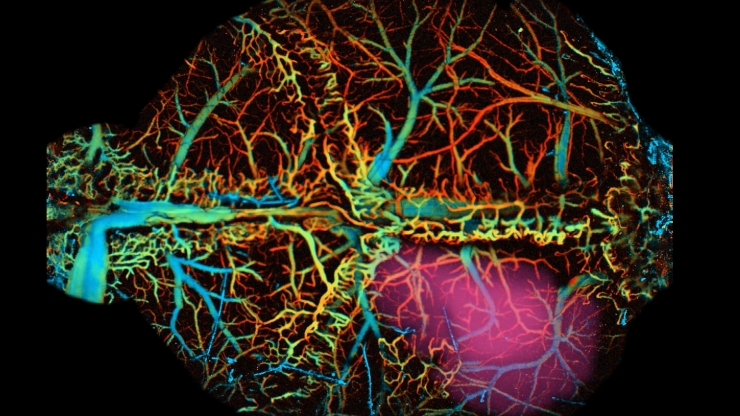
\includegraphics[width=0.4\textwidth]{figures/example_figure.jpeg}
  \caption{Integer feugiat libero ut malesuada sollicitudin. In ornare, enim quis aliquet volutpat.} 
\end{figure}


Lorem ipsum dolor sit amet, consectetur adipiscing elit. Phasellus sagittis neque id ex faucibus pellentesque. Nam nulla sem, porta at mollis vitae, pretium ac lectus \cite{chaplot2020learning}. Aenean varius erat leo, sit amet maximus sem fringilla id. In nibh sem, sodales eget placerat nec, elementum vel lorem. Cras vel odio odio. Integer feugiat libero ut malesuada sollicitudin. In ornare, enim quis aliquet volutpat, justo nisl consequat ipsum, quis feugiat sem mauris id ipsum. Aenean tincidunt vulputate lectus a congue. Ut in lorem ante. Nulla fermentum libero magna, faucibus consectetur lacus maximus et. Nunc dui urna, consectetur ut convallis eu, egestas a augue. Aliquam erat volutpat. Fusce blandit sapien sed ex sagittis consequat. Duis eleifend ipsum non turpis lacinia ultrices.

Aliquam urna neque, lacinia eu faucibus eget, placerat ac odio. Integer sed orci justo. Mauris placerat magna eget quam tincidunt, non suscipit ipsum venenatis. Proin consequat scelerisque turpis ac mattis. In velit urna, pellentesque nec nibh consequat, ullamcorper viverra enim. Nullam tempus ante vel quam egestas pellentesque. Vivamus odio nibh, tristique vitae justo quis, ullamcorper dignissim felis \cite{chaplot2020object}.

Nam dictum risus nisl, id eleifend urna condimentum et. Duis ut risus aliquet, semper quam sit amet, dignissim dui. Vestibulum ut ante scelerisque, scelerisque odio vel, malesuada magna. Proin enim mi, rutrum at condimentum vitae, placerat quis quam. Aliquam lacus sem, aliquam sed placerat volutpat, faucibus quis felis. Nunc ultrices ut turpis non tempus. Phasellus lacus felis, ultrices nec risus eu, fermentum sodales tellus.

% ---------- Method and Deliveries ----------
\section{Method and Deliveries}

\subsection{Proposed Neural Architecture}

Nam dictum risus nisl, id eleifend urna condimentum et. Duis ut risus aliquet, semper quam sit amet, dignissim dui. Vestibulum ut ante scelerisque, scelerisque odio vel, malesuada magna. Proin enim mi, rutrum at condimentum vitae, placerat quis quam. Aliquam lacus sem, aliquam sed placerat volutpat, faucibus quis felis. Nunc ultrices ut turpis non tempus. Phasellus lacus felis, ultrices nec risus eu, fermentum sodales tellus \cite{elfes1987sonar}.

\subsubsection{Mapper Architecture}


Lorem ipsum dolor sit amet, consectetur adipiscing elit. Phasellus sagittis neque id ex faucibus pellentesque. Nam nulla sem, porta at mollis vitae, pretium ac lectus. Aenean varius erat leo, sit amet maximus sem fringilla id. In nibh sem, sodales eget placerat nec, elementum vel lorem. Cras vel odio odio. Integer feugiat libero ut malesuada sollicitudin. In ornare, enim quis aliquet volutpat, justo nisl consequat ipsum, quis feugiat sem mauris id ipsum. Aenean tincidunt vulputate lectus a congue. Ut in lorem ante. Nulla fermentum libero magna, faucibus consectetur lacus maximus et. Nunc dui urna, consectetur ut convallis eu, egestas a augue. Aliquam erat volutpat. Fusce blandit sapien sed ex sagittis consequat. Duis eleifend ipsum non turpis lacinia ultrices.

Aliquam urna neque, lacinia eu faucibus eget, placerat ac odio. Integer sed orci justo. Mauris placerat magna eget quam tincidunt, non suscipit ipsum venenatis. Proin consequat scelerisque turpis ac mattis. In velit urna, pellentesque nec nibh consequat, ullamcorper viverra enim. Nullam tempus ante vel quam egestas pellentesque. Vivamus odio nibh, tristique vitae justo quis, ullamcorper dignissim felis.

Nam dictum risus nisl, id eleifend urna condimentum et. Duis ut risus aliquet, semper quam sit amet, dignissim dui. Vestibulum ut ante scelerisque, scelerisque odio vel, malesuada magna. Proin enim mi, rutrum at condimentum vitae, placerat quis quam. Aliquam lacus sem, aliquam sed placerat volutpat, faucibus quis felis. Nunc ultrices ut turpis non tempus. Phasellus lacus felis, ultrices nec risus eu, fermentum sodales tellus.

\subsubsection{Planner Architecture}


Aliquam urna neque, lacinia eu faucibus eget, placerat ac odio. Integer sed orci justo. Mauris placerat magna eget quam tincidunt, non suscipit ipsum venenatis. Proin consequat scelerisque turpis ac mattis. In velit urna, pellentesque nec nibh consequat, ullamcorper viverra enim. Nullam tempus ante vel quam egestas pellentesque. Vivamus odio nibh, tristique vitae justo quis, ullamcorper dignissim felis.

\subsection{Proposed Roadmap and Implementation}
Lorem ipsum dolor sit amet, consectetur adipiscing elit. Phasellus sagittis neque id ex faucibus pellentesque. Nam nulla sem, porta at mollis vitae, pretium ac lectus. Aenean varius erat leo, sit amet maximus sem fringilla id. In nibh sem, sodales eget placerat nec, elementum vel lorem. Cras vel odio odio. Integer feugiat libero ut malesuada sollicitudin. In ornare, enim quis aliquet volutpat, justo nisl consequat ipsum, quis feugiat sem mauris id ipsum. Aenean tincidunt vulputate lectus a congue. Ut in lorem ante. Nulla fermentum libero magna, faucibus consectetur lacus maximus et. Nunc dui urna, consectetur ut convallis eu, egestas a augue. Aliquam erat volutpat. Fusce blandit sapien sed ex sagittis consequat. Duis eleifend ipsum non turpis lacinia ultrices.

Aliquam urna neque, lacinia eu faucibus eget, placerat ac odio. Integer sed orci justo. Mauris placerat magna eget quam tincidunt, non suscipit ipsum venenatis. Proin consequat scelerisque turpis ac mattis. In velit urna, pellentesque nec nibh consequat, ullamcorper viverra enim. Nullam tempus ante vel quam egestas pellentesque. Vivamus odio nibh, tristique vitae justo quis, ullamcorper dignissim felis.

Nam dictum risus nisl, id eleifend urna condimentum et. Duis ut risus aliquet, semper quam sit amet, dignissim dui. Vestibulum ut ante scelerisque, scelerisque odio vel, malesuada magna. Proin enim mi, rutrum at condimentum vitae, placerat quis quam. Aliquam lacus sem, aliquam sed placerat volutpat, faucibus quis felis. Nunc ultrices ut turpis non tempus. Phasellus lacus felis, ultrices nec risus eu, fermentum sodales tellus.

% No problem nor solution thereof ever exists in a vacuum.
% Cite~\cite{example} relevant work here to support your choice of problem and proposed approach, and explain about how your solution differs from existing ones.


% ---------- Discussion ----------
\section{Discussion}
The main challenge posed by our approach is the compute resource limitations we are subject to. Even with a promising architecture we might not get to good performance because of limited compute. To address this, we propose using low resolution images, maps and buffers wherever possible. It is important to note this may require adding modifications to mid-level encoders which are meant for \texttt{256x256} RGB images. \\

Furthermore we hypothesize that using supervised training to initialize well chosen parts of our network can allow us to increase the learning speed of our algorithm. The most straightforward approaches would be:
\begin{enumerate}
    \item train the mapper decoder on ground truth free space
    \item train the RL policy using ground truth free space as input
\end{enumerate}

The decoupled training procedure above is only thought of as a way to initialize the network weights. We plan to train our network "end-to-end" (while fixing the mid-level representations networks) using PPO.
\printbibliography

\end{document}
